% =====================================================================
%  CH 12-13 : Souveraineté cryptographique · Cérémonies et kit du terrain
%  v0.6.0 (D133) — sources scellées : v06/I/README.md (axe 3),
%  v06/I/CF2/README.md (axe 2), v06/I/CF3/README.md (axe 4, D121).
%  Le texte ci-dessous est la synthèse NORMATIVE ; l'arbre signé v06/I/
%  reste la source de vérité sous le sceau de l'Intention.
% =====================================================================
\section{Souveraineté cryptographique — le programme v0.6.0}\label{sec:souverainete}

La menace fondatrice est nommée depuis D84 : \emph{l'expropriation} — un tiers (typ.
l'employeur) qui s'empare du binaire, du dépôt, voire des clés du poste. La barrière
juridique (licence BSL 1.1) répond aux tribunaux ; la barrière cryptographique répond à
la machine. Le programme a été décidé en trois axes (D85--D87, 28/10), un quatrième est
né du terrain (D121) ; à la passation, l'état est le suivant :

\begin{table}[htbp]
\centering\small
\caption{Le programme de souveraineté cryptographique — état à la passation v0.6.0 (D133).}
\label{tab:axes}
\begin{tabularx}{\textwidth}{@{}l Y Y@{}}
\toprule
\textbf{Axe} & \textbf{Mécanisme livré} & \textbf{État} \\
\midrule
1 · Attestation de non-exfiltration (D85) & quote vérifiable TPM 2.0/SGX du code
manipulant le coffre ; le coffre refuse de déverrouiller sans quote (fail-closed) &
\textbf{exigence consignée} — l'infrastructure sans TEE ne peut pas la satisfaire et
le dit \\
2 · Interrupteur d'homme mort (D86) & clé maîtresse CF2 jamais stockée entière (Shamir,
cinq gardes seuil 3) ; sentinelle à double seuil ; destruction des fragments ; PORTE
D120 & \textbf{livré, prouvé terrain} — chaîne réelle migrée CF1 $\to$ CF2 le 31/10/2026 \\
3 · Filigrane de l'Intention (D87) & chaque arbre de couche I condensé puis signé par
la clé Ed25519 \emph{hors-ligne} du développeur ; build et chemin de patch refusent
une couche I non signée & \textbf{livré, prouvé terrain} — treize arbres signés ;
re-cérémonie réelle D126, cérémonies d'ère M8 (12 arbres, D162/D163) et M9 (13
arbres, D166/D168) passées sur pièces — verifier 13 arbres VERTS \\
4 · Serrure piégée (D121) & coffre CF3 : clé utilisateur invariable, moitiés
serrure/piège fraîches à chaque époque, piège sur média séparé, cycle en deux actes,
sentinelle instantanée par invocation & \textbf{livré, prouvé terrain} — chaîne réelle
migrée CF2 $\to$ CF3 le 30--31/10/2026, époque 1, verdict à froid VERT \\
\bottomrule
\end{tabularx}
\end{table}

Les sources normatives de ce chapitre vivent \textbf{sous le sceau de l'Intention} :
\code{v06/I/README.md} (axe 3), \code{v06/I/CF2/README.md} (axe 2) et
\code{v06/I/CF3/README.md} (axe 4) — la même signature Ed25519 couvre le programme
entier. Le présent chapitre en est la synthèse de spécification ; en cas de divergence,
l'arbre signé fait foi.

\paragraph{Positionnement du programme.} La priorité fut donnée aux axes 2 et 3 après le
scellage 0.5.0 de M4 — ils touchent les disciplines de rotation et de garde existantes
et devaient s'intégrer aux cérémonies de lignée ; l'axe 4 (D121) est né du terrain en
cours de déploiement et a été servi avant la migration du coffre réel, exactement dans
l'ordre qui rendait la migration définitive. L'axe 1 suit la disponibilité d'une
infrastructure à racine de confiance matérielle : l'exigence est consignée, l'attente
est dite. La hiérarchie des clés qui en découle — phrase de lignée (chiffre les
enveloppes, vol au repos), graine Ed25519 en ligne (signe les cartes, les faits), clé I
hors-ligne (signe l'intention, la volonté), clave du coffre (le secret réparti) — se
lit comme la réponse machine à la barrière juridique de la BSL : la licence pour les
tribunaux, les preuves pour la machine.

\subsection{La hiérarchie des gardes — quatre secrets, quatre menaces}\label{sec:gardes}

La souveraineté n'est pas un secret unique mais une \textbf{hiérarchie} : chaque garde
répond à une menace que les autres ne couvrent pas, et aucune ne duplique la preuve
d'une autre (défaut X2 — un mécanisme de garde qui s'exempte de lui-même serait une
contrebande).

\begin{table}[htbp]
\centering\small
\caption{Les quatre gardes de la souveraineté.}
\label{tab:gardehi}
\begin{tabularx}{\textwidth}{@{}l Y Y@{}}
\toprule
\textbf{Garde} & \textbf{Menace couverte} & \textbf{Où elle vit} \\
\midrule
Phrase de lignée & chiffre les enveloppes de carte — vol du dépôt au repos & en tête
du développeur, séquestre D183/D223 (cinq parts Shamir à seuil trois, la
reconstitution à froid — la phrase en aucun dépôt) \\
Graine Ed25519 en ligne & signe les cartes — atteste les \textsc{faits} (les octets
scellés) & dépôt du développeur (jamais confiée au bac à sable, D30) \\
Clé I hors-ligne & signe l'intention — atteste la \textsc{volonté} (le droit de faire
évoluer) & support physique hors machine ; le dépôt ne voit que la clé publique \\
Clave du coffre (CF2/CF3) & le secret maître du coffre — expropriation du poste vivant &
CF2 : répartie par Shamir, cinq gardes, seuil 3, jamais entière ; CF3 : moitié piège sur
média séparé, jamais sur la machine \\
\bottomrule
\end{tabularx}
\end{table}

Le code volé ne peut pas \emph{évoluer} (axe 3) ; le dépôt volé ne peut pas être
\emph{déverrouillé} (axes 2 et 4) ; la licence BSL donne aux tribunaux la lecture
juridique du même état de fait.

\subsection{CF2 — la clé maîtresse répartie (D86)}\label{sec:cf2}

Le secret maître \textbf{M} (32 octets CSPRNG) n'est \emph{jamais} écrit entier —
nulle part, jamais. Il vit reconstitué en RAM le temps d'un déverrouillage, puis est
effacé. Le conteneur \code{TRIADE-CF2} dérive sa clé de chiffrement de M par
HKDF-SHA256 à contexte dédié (\code{coffre=v2} — nul chevauchement avec CF1 ni avec les
fragments de carte) ; le champ \code{verif} (16 octets) est la vérification nommée de
toute reconstitution, l'AEAD re-verrouillant derrière.

\paragraph{Le découpage Shamir (normatif).} Champ GF($2^8$), polynôme générateur
\textbf{0x11B} (celui d'AES). Pour chacun des 32 octets de M, un polynôme distinct de
degré $T-1$ à coefficients \emph{frais du CSPRNG} (jamais réutilisés d'un octet à
l'autre) ; le fragment $j$ porte le vecteur des évaluations $f_j$. Indices $x_j \in
\{1 \dots N\}$ distincts et non nuls ; bornes $2 \le T \le N \le 255$ ; \textbf{T = 1
refusé} (aucune distribution : la garde serait une clé unique, alternative rejetée par
D86). Reconstitution par interpolation de Lagrange en $x = 0$ sur $T$ fragments
\emph{valides} distincts, vérifiée contre \code{verif} avant toute interprétation.
\textbf{Sous le seuil, la sécurité est informationnelle} : tout $M'$ de 32 octets reste
compatible avec les fragments présents — la destruction des fragments est une mort, pas
une révocation.

\paragraph{Fragments et gardes.} Le format fragment est ASCII autodescriptif,
transportable \emph{sur papier} (l'exfiltration d'un fragment est un vol physique — hors
modèle) :

\begin{lstlisting}
TRIADE-CF2-FRAG v1
coffre: <sel HKDF du conteneur, 64 hex - identite STABLE du coffre>
x: <indice, decimal>
seuil: t=3/n=5
fragment: <64 hex - 32 o>
tag: <16 hex - sha256("TRIADE-CF2-frag" || x || fragment) tronque>
\end{lstlisting}

Le fragment est lié au \emph{sel} du coffre (identité stable par construction) et
jamais à l'empreinte de l'en-tête : le nonce est frais à chaque écriture, une liaison à
l'en-tête invaliderait les copies papier à chaque mutation — faute dénoncée par le
parcours CLI complet et consignée (D106). Une garde est un répertoire distinct portant
un fragment (mode 0700) ; en production, ACL distinctes et supports séparés. Valeurs de
l'arbitrage terrain : \textbf{N = 5, T = 3} — brûler les cinq gardes machine tue le
coffre ; la \textbf{relève exige T copies hors-ligne} (trois à seuil 3 : deux copies
laisseraient le coffre mort, l'autotest le prouve par restauration partielle refusée ;
erratum D121 consigné).

\begin{lstlisting}
magic "TRIADE-CF2" (10 o) . version u16 (1) .
champs longueur-prefixee u16 : hachage (sha256), kdf (hkdf-sha256),
                       chiffrement (xchacha20poly1305),
                       date ISO-8601 UTC, shamir ("t=3/n=5") .
sel HKDF 32 o (aleatoire a l'init) . nonce 24 o (frais a CHAQUE
ecriture) . empreinte sha256 du chiffretexte 32 o .
verif 16 o = sha256(HKDF(M, sel, info "cf2=verif")) tronque .
chiffretexte : XChaCha20-Poly1305(JSON base, K, AAD = tout ce qui precede)
   avec K = HKDF-SHA256(M, sel du conteneur, info "coffre=v2", L=32)
\end{lstlisting}

La base déchiffrée est le \emph{même} JSON que CF1 — la migration ne traduit rien
(\code{\{format, protocole, cree, modifie, description, projets\}}). Toute anomalie de
parsing, d'algorithme (liste blanche de l'en-tête), d'empreinte, de \code{verif} ou de
tag AEAD est un refus terminal — rien n'est interprété (fail-closed) ; écriture
atomique (tmp + \code{os.replace} + fsync, 0600, répertoire 0700).

\paragraph{La sentinelle, puis la porte D120.} La sentinelle CF2 est un processus
userland long terme qui surveille la couche C (jamais les gardes ni le conteneur), à
\textbf{double seuil} : processus hors liste blanche \emph{et} lecture de contenu — deux
signaux indépendants requis, la fausse alerte étant une perte auto-infligée. Moteur
laboratoire : inotify + attribution \code{/proc} (latence mesurée 0,05 s, borne 2 s) ;
moteur de production Windows : SACL + journal 4663 ou ETW — \emph{exigence consignée},
le bac à sable ne pouvant la satisfaire. La demande du terrain (D120) — « si le
déverrouillage est tenté et qu'elle n'est pas lancée, tous nos efforts sont inutiles » —
a posé la \textbf{PORTE} : le coffre exige une sentinelle vivante pour déverrouiller ;
sur plateforme sans moteur, la porte \emph{avertit nommément} à chaque déverrouillage
(« SANS sentinelle ») jusqu'au moteur réel — l'ère intermédiaire est dite, pas cachée.
La destruction (\code{bruler}) — trois passes d'écrasement, troncature, renommage
aléatoire, unlink, fsync — laisse un \textbf{procès-verbal} nommant le déclencheur ;
le conteneur et les gardes vides restent sur place : le PV dit la mort, la vérification
la confirme. La restauration (\code{restaurer}) est \emph{atomique} : toute anomalie et
rien n'est écrit — une remise partielle serait un coffre menteur.

\subsection{CF3 — la serrure à triple scellement (D121)}\label{sec:cf3}

CF3 répond à deux demandes du terrain servies ensemble : « plutôt qu'une sentinelle
externe, une serrure du coffre piégée » et « une vulnérabilité réside durant le temps
où la session est ouverte ». L'exigence D120 \emph{reste} — réalisée \textbf{par
invocation au lieu de résidence} : le démon résident était usurpable (faux heart-beat,
borne D120 consignée) ; la sentinelle instantanée ne dépend d'aucun état de machine
falsifiable — \emph{le piège est le témoin, et il est hors machine}.

\paragraph{Les trois éléments (normatif).} \textbf{K\_user} : la clé de l'utilisateur,
\code{Argon2id(phrase, sel\_argon)} — 32 octets, paramètres miroir CF1 (65536 Kio,
3 itérations, parallélisme 1) — \textbf{invariable à travers les époques} ;
\textbf{S\_serrure} : la moitié « serrure », 32 octets frais du CSPRNG à chaque époque,
dans l'en-tête clair du conteneur ; \textbf{S\_piège} : la moitié « piège », 32 octets
frais à chaque époque, \emph{exclusivement sur un média séparé}. L'\textbf{époque}
(u64, posée à 1, incrémentée à chaque clôture) est l'horloge de la métamorphose et le
témoin anti-retour ; \textbf{H\_projet} (sha256 de l'état scellé) est le liant de la clé
de clôture au contenu. Trois pièges de l'intuition d'origine, désamorcés et consignés :
un hash de projet est public (il \emph{lie}, il ne protège pas — l'entropie vient de
K\_user, S\_serrure, S\_piège) ; le piège ne doit pas être dérivable de la serrure
(deux aléas indépendants) ; détruire sur mauvaise clé serait un DoS offert (la phrase
erronée est bénigne, seule la falsification \emph{prouvée} détruit — dans les DEUX phases : la sentinelle court sur le conteneur canonique, la destruction locale sur falsification prouvée pendant une session ouverte comprise, jamais le média ni les fragments ; le modèle formel v0.15.3 offre la règle aux deux phases, l'écart d'approximation de la v0.15.0 fermé par l'extension 5ey7gmjra).

\paragraph{Dérivation et conteneur.}
$\mathrm{KEK} = \mathrm{HKDF\text{-}SHA256}(\mathrm{ikm} =
K_{user} \| S_{serrure} \| S_{piege};\ \mathrm{salt} = sel_{hkdf};\ \mathrm{info} =
\text{«\,triade-CF3/v1\,»} \| \acute{e}poque_{le64} \| H_{projet})$,
puis XChaCha20-Poly1305 (nonce 24 o, AAD = tout l'en-tête jusqu'au nonce inclus). Le
champ \textbf{verif} rend l'essai-hors-ligne impossible au voleur de la machine seule :
$verif = \mathrm{sha256}(\mathrm{HKDF}(K_{user} \| V_{piege};\ info =
\text{«\,triade-CF3/verif/v1\,»}))[:16]$, où $V_{piege}$ est une valeur
\emph{publique} portée par le fichier piège — le conteneur seul ne suffit pas à tester
des phrases.

\begin{lstlisting}
"TRIADE-CF3" 10 o | version u16 (=1) | epoque u64 | H_projet 32 o |
sel_argon 16 o | params (t,m,p : u32x3) | sel_hkdf 32 o | S_serrure 32 o |
nonce 24 o |                       <- fin de l'AAD (168 o)
empreinte 32 o = sha256(chiffretexte) | verif 16 o |
chiffretexte = AEAD(clair, aad, nonce, KEK)
\end{lstlisting}

\paragraph{Le fichier piège.} Un fichier texte ASCII \emph{par époque}, sur le média
séparé (le sachet du kit, à côté des fragments hors-ligne) :
\code{piege-CF3-epoque-<époque>.txt}. Une clôture \textbf{ajoute} le piège N+1 et ne
ronge jamais les pièges des époques passées (l'ancien piège est la relève du canonique
précédent) ; seul le créneau N+1 peut être remplacé — par le rejeu d'une clôture
interrompue. Un média du piège par coffre (le sachet est individuel). Le \code{tag}
nomme la corruption sans divulguer ; borne consignée : un piège entièrement forgé se
présente comme une phrase erronée — bénin, refus nommé, jamais de destruction. Le média
peut demain être une clé USB à bouton physique (FIDO2) : seul le support change.

\paragraph{La sentinelle instantanée — l'ordre est la loi.} À tout acte qui déverrouille
(ouvrir, clôture, \code{verifier}, re-lecture à froid) : (1) piège \emph{présent} —
absent, le déverrouillage est \emph{impossible} (fail-closed), rien n'est lu, rien ne
brûle ; (2) piège \emph{intègre} (tag) — invalide, refus nommé \emph{sans} destruction
(le média est hors limite de confiance) ; (3) \emph{cohérence des champs publics} —
époque du piège = époque du conteneur (divergence : « piège PÉRIMÉ », refus
anti-retour), H\_projet du piège = H\_projet du conteneur (divergence : piège d'un autre
coffre) ; (4) \emph{phrase} (verif) — diverge : réessai à délai croissant (1, 2, 4 s,
plafond 8 s), \emph{jamais} de destruction ; (5) \emph{AEAD + étiquette} — échec après
1--4 verts : falsification ou corruption \emph{prouvée} côté machine $\to$ destruction
locale + PV + journal. L'étiquette est vérifiée : le clair déchiffré doit hacher vers le
H\_projet de l'en-tête — c'est ce qui ferme la course de clôture. Un échec nomme son
étape ; les suivantes ne courent pas.

\paragraph{Le cycle en deux actes.} \textbf{Acte I — ouverture} : phrase + piège $\to$
sentinelle instantanée $\to$ clair $\to$ \emph{brouillon} chiffré sur disque sous une
clé de session éphémère K\_session (RAM de l'objet Session seule) ; K\_user, KEK,
moitiés effacés ; média \emph{débranché} (geste humain consigné) ; le canonique n'est
\emph{jamais} réécrit pendant la session. \textbf{Session} : travail sur le brouillon ;
une panne tue K\_session avec le processus — le brouillon devient déchet indéchiffrable,
le canonique reste scellé : \emph{une panne auto-nettoie}. \textbf{Acte II — clôture} :
média rebranché, phrase \emph{retapée} (une faute de frappe est bénigne) ; moitiés
fraîches, époque N+1, KEK de clôture dérivé \emph{avec} H\_final (lié au contenu) ;
écriture du piège N+1 (additive) puis du conteneur en \emph{staging} ; \textbf{re-lecture
à froid} du staging par la sentinelle complète — verte : remplacement atomique
(\code{os.replace}) ; échec : staging détruit, canonique et brouillon intacts, la
clôture est rejouable. Checksum court de 8 hex \emph{affiché} : l'humain recoupe avec
sa carte.

\paragraph{Anti-retour-en-arrière et bornes.} Le roll-back restaure un \emph{couple}
cohérent (conteneur N + piège N) — l'AEAD passerait seul. Trois miroirs d'époque, du
plus faible au plus fort : journal local (contrôle automatique, effaçable par un
attaquant admin), \textbf{carte papier du sachet} (checksum consigné à la main à chaque
clôture, indécevable par logiciel), journal Git (poussé, hors machine). Bornes assumées
et dites : un attaquant admin contrôlant la machine \emph{pendant} l'acte voit la phrase
— le rayon est borné à une époque (moitiés neuves à chaque clôture) ; le contenu de la
session reste lisible par un malware présent pendant le travail — sessions courtes,
re-verrouillage rapide ; l'affichage du checksum ne protège que s'il est regardé.

\begin{table}[htbp]
\centering\small
\caption{Les trois générations du coffre-fort — lecture comparative.}
\label{tab:comparatif}
\begin{tabularx}{\textwidth}{@{}l Y Y Y@{}}
\toprule
 & \textbf{CF1 (D75)} & \textbf{CF2 (D86)} & \textbf{CF3 (D121)} \\
\midrule
Cérémonie de la clé & une phrase, dérivation Argon2id & secret maître M réparti par
Shamir, reconstitué en RAM le temps d'un acte & trois éléments : K\_user invariable,
S\_serrure et S\_piège frais à chaque époque \\
Ce qui est exigé pour déverrouiller & la phrase & T fragments valides (seuil) & la
phrase \emph{et} le piège d'époque égale — sinon l'acte est impossible \\
Sentinelle & — & démon résident à double seuil, puis PORTE D120 & instantanée, par
invocation, à chaque acte — la serrure est le témoin \\
Session & lecture/écriture directes & lecture/écriture directes, M effacé après usage &
cycle en deux actes : brouillon sous K\_session, canonique jamais réécrit \\
Anti-retour & — & monotonie du conteneur & trois témoins d'époque (journal local,
carte papier, journal Git) \\
Falsification prouvée & refus (AEAD) & refus (AEAD + verif) & destruction locale + PV —
jamais le média ni les fragments \\
Relève si la machine brûle & la phrase — la garde d'époque D81 amendée le
19 novembre 2026 : le séquestre 5/3, la reconstitution à froid de TROIS parts
(D223) & T copies hors-ligne des fragments & le sachet : pièges d'époque + carte papier \\
\bottomrule
\end{tabularx}
\end{table}

\subsection{Le sceau de l'Intention (D87)}\label{sec:sceauI}

Quatorze arbres de couche I vivent sous le sceau — les lignées m0 à m8 (le domaine
\code{sys} depuis l'ère M8), l'arbre \code{tls13} (le domaine TLS 1.3 pur depuis
l'ère M9), \code{demo}, \code{terrain}, l'arbre \code{loupe} (le domaine M10, entré
à la table canonique par la cérémonie d'ère du TGN, D171/D177) et l'arbre des axes
eux-mêmes (\code{v06/I}) : la spécification qui définit le sceau est la première couche I
qu'il garde. Chaque ère qui ouvre un arbre nomme sa dette de cérémonie à la
naissance (D166, règle 8) : le registre figé étendu et l'arbre neuf exigent la clé
hors-ligne avant tout build — la charge se prépare au geste qui sert la main du
développeur (D168), et la continuité de la clé se prouve par le déterminisme
Ed25519 (D163) : re-signer les arbres inchangés redonne exactement les signatures
déposées. L'ère du TGN (le domaine \code{loupe}, D171) a suivi la même discipline :
la dette du quatorzième arbre fut nommée à la naissance puis SOLDÉE par la cérémonie
passée sur pièces (D177 : le garde à QUATORZE arbres, l'état « reelle » tenant — le
build de l'ère a vécu). Pour chaque arbre,
le \textbf{manifeste} est le texte
canonique (UTF-8, LF, tri lexicographique déterministe du chemin relatif POSIX) ; chaque
ligne fichier porte le SHA-256 du contenu \emph{canonique LF} — la représentation du
checkout (Windows \code{autocrlf} porte CRLF) n'est pas l'intention (D115, appris de la
cérémonie terrain D113 dont les empreintes CRLF dénonçaient les dix arbres à froid).
L'\textbf{empreinte d'arbre} est le SHA-256 du manifeste entier ; la signature
\textbf{Ed25519} (RFC 8032) couvre l'empreinte — un message de 32 octets, imprimable
sur papier : la cérémonie hors-ligne manipule des charges utiles de quelques lignes
hexadécimales, jamais le dépôt.

\begin{lstlisting}
TRIADE-SCEAU-I v1
arbre: m4
artefact: proxy.exe
balise: 0.5.0
fichiers: 12
sha256:<64 hexdecimaux minuscules>  tls-01-nom-utf16.md
sha256:<64 hexdecimaux minuscules>  tls-02-verdicts.md
...
\end{lstlisting}

Règles du manifeste : tous les fichiers réguliers de l'arbre sont listés (un ajout non
signé est un diff d'intention, refusé comme une modification) ; chaque ligne porte le
SHA-256 du contenu canonique LF, hexadécimal minuscule, deux espaces après le condensé ;
répertoires vides, liens symboliques et fichiers spéciaux : refus de préparation
(fail-closed) ; l'empreinte d'arbre est le SHA-256 du manifeste \emph{entier} — aucun
champ n'est hors signature.

La cérémonie hors-ligne est \emph{autoportée} (stdlib Python seule, aucune dépendance,
aucun réseau — exécutable sur toute machine 3.8+ y compris hors ligne) :
\code{generer} (graine Ed25519, le fichier est la remise), \code{signer} (chaque
signature vérifiée avant écriture), \code{verifier} (audit autonome). Le flux est
\emph{air-gap} : le dépôt produit \code{a-signer.txt}, la clé et les signatures
reviennent au dépôt (\code{v06/sceau-I/}) — le dépôt ne voit jamais la graine. La
garde vit dans la source des chaînes : \code{build\_m4.py} et \code{build\_terrain.py}
appellent la garde au plus tôt — un arbre divergé de sa signature \emph{refuse le build} ;
tout script qui modifie une couche I doit appeler la garde en sortie — le diff non signé
est refusé. \code{verifier} rend ses codes nommés : 0 (tout vert), 10 (arbre divergé —
diff d'intention non signé), 11 (signature invalide), 12 (dépôt incohérent). Ce que la
garde n'est pas : elle ne protège pas contre la réécriture intégrale arbre + manifeste +
signature + clé publique — cette menace appartient à la phrase de lignée et au dépôt git
signé ; trois gardes, trois menaces.

\subsection{Le niveau du coffre neuf — un arbitrage du développeur (D137)}\label{sec:initniveau}

La chaîne CF1 $\to$ CF2 $\to$ CF3 est le chemin \emph{historique} du coffre réel —
né CF1 (D75), armé CF2 (D86), scellé CF3 (D121), migré par cérémonies successives ;
elle n'est plus un rang de naissance. La v0.6.0 fixait la règle « un coffre neuf
naît CF3 » (\code{init} direct, époque 1, média du piège dès le premier jour) ; la
v0.6.1 revient sur cet arbitrage : \textbf{le niveau de sécurité d'un coffre neuf —
CF1, CF2 ou CF3 — est choisi par le développeur lors de la création de son projet de
développement} (D137). Imposer CF3 par défaut risque d'être trop contraignant selon
le projet : le niveau le plus fort exige un média de piège dès le premier jour, le
cycle en deux actes à chaque session, le sachet physique et sa carte — la contrainte
se justifie quand le secret la mérite, pas pour tout projet.

\begin{table}[htbp]
\centering\small
\caption{Les trois naissances — l'acte de création détermine le niveau et ses obligations.}
\label{tab:naissances}
\begin{tabularx}{\textwidth}{@{}l >{\raggedright\arraybackslash}p{4.6cm} Y@{}}
\toprule
\textbf{Niveau} & \textbf{Acte de création} & \textbf{Ce qui vient avec} \\
\midrule
CF1 & \code{coffre\_fort.py init} & conteneur chiffré à phrase (D75) ; la garde
de la phrase à l'arbitrage du développeur (D137 — la garde active
D223 : le séquestre à seuil, la reconstitution à froid de trois
parts, la phrase en AUCUN dépôt ; l'histoire D81 datée du 4 au
19 novembre 2026) ; relève simple \\
CF2 & \code{coffre\_fort.py init} puis cérémonie \code{coffre\_cf2.py migrer} —
l'\code{init} direct de CF2 demeure un outil de LABORATOIRE, la spécification
scellée CF2 (§ 12 : phase laboratoire / cérémonie réelle) fait foi & clé maîtresse
répartie Shamir (N gardes, seuil T), T copies hors-ligne, liste blanche,
sentinelle/porte D120 \\
CF3 & \code{coffre\_cf3.py init} & époque 1, média du piège dès le premier jour,
cycle en deux actes, sentinelle par invocation, sachet + carte papier
(§\ref{sec:ceremonies}) \\
\bottomrule
\end{tabularx}
\end{table}

\paragraph{Le guide de l'arbitrage (recommandation, pas contrainte).} CF1 suffit
quand la menace est le vol au repos du poste seul et que la simplicité de relève
prime — prototype, projet jetable, secrets reproductibles ; CF2 quand la garde doit
être partagée ou survivre au maître — quorum, relève à plusieurs ; CF3 pour les
secrets maîtresses d'un projet vivant sous menace d'expropriation — la référence
demeure le coffre réel de TRIADE, né CF1 et monté à CF3 par cérémonies. La montée
n'est jamais bloquée : \textbf{la chaîne de migration CF1 $\to$ CF2 $\to$ CF3 reste
disponible à tout moment} — les besoins grandissent, le coffre suit ; la descente de
niveau n'existe pas (\code{bruler} demeure l'acte de fin de vie). Le niveau choisi se
consigne au journal des décisions du projet avec sa raison — un arbitrage muet serait
un contrat non écrit (§\ref{sec:taxonomie}).

\paragraph{La sentinelle, au niveau CF3.} La question du terrain — \emph{puisqu'un
coffre né CF3 porte sa sentinelle dès la création, celle-ci ne devient-elle pas
inutile ?} — garde sa réponse normative : la sentinelle de CF3 n'est pas un composant
qu'on peut oublier de lancer, c'est la serrure elle-même ; l'exigence D120
(« indispensable au déverrouillage ») est réalisée \emph{par construction}, sans
démon résident ni moteur de plateforme à attendre. Ce qui demeure obligatoire, niveau
par niveau : CF1 — la garde de la phrase à l'arbitrage du développeur (D137 ;
la garde active D223 : la reconstitution à froid de trois parts du
séquestre, la phrase en AUCUN dépôt — le refus nommé de l'écriture
de dépôt) ; CF2 — les T copies hors-ligne et
la liste blanche ; CF3 — le média du piège (sans S\_piège, le déverrouillage est
\emph{impossible}, pas seulement refusé) et la discipline du sachet
(§\ref{sec:ceremonies}).

\subsection{Bornes honnêtes consolidées du programme}\label{sec:bornes}

Le modèle de menace dit ses limites — aucune cachée :

\begin{itemize}
\item \textbf{Attaquant admin/noyau pendant un acte} : il voit la phrase, peut
photographier le média branché et forger un conteneur complet ; le rayon est borné à
\emph{une} époque (moitiés neuves à chaque clôture). Cérémonie sur machine propre,
sessions courtes — c'est la parade opérationnelle, pas une garantie logicielle.
\item \textbf{Zéroïsation au mieux de Python} : \code{bytearray} effacé + \code{del} ;
la garantie native (\code{SecureZero\allowbreak Memory}) est une affaire de déploiement Windows —
limite consignée depuis CF2.
\item \textbf{Sentinelle CF2 tuable} : l'adversaire utilisateur peut tuer le démon avant
destruction (borne D86) ; le heart-beat rend la mort \emph{visible}. CF3 supprime la
classe du risque : plus de démon à tuer — l'exigence vit dans la serrure.
\item \textbf{Lecture non attribuée} (CF2) : une lecture de fichier $< \sim$10 ms peut
refermer avant attribution — journalée, non brûlée ; une exfiltration réelle (copie
d'arbre, secondes) est garantie attrapée.
\item \textbf{CoW / instantanés} : l'écrasement logique ne tue pas les copies physiques
sur ZFS/btrfs ; ext4/overlayfs au laboratoire, TRIM au déploiement (exigence
consignée).
\item \textbf{Carte papier regardée} : l'affichage du checksum ne protège que s'il est
regardé — le verdict à froid re-exécuté par la machine est le filet.
\item \textbf{Axe 1 (TEE) non satisfait} : l'attestation de non-exfiltration exige une
racine de confiance matérielle ; l'infrastructure actuelle ne peut pas la fournir et le
dit — exigence consignée, pas promesse.
\end{itemize}

\section{Les cérémonies et le kit du terrain}\label{sec:ceremonies}

Les cérémonies de la souveraineté sont des \emph{actes du maître} : le bac à sable ne
touche jamais le conteneur ni les phrases réels (discipline D105). L'outillage les guide
sans les réimplémenter — il lance les vérités vivantes et leur sortie coule à l'écran.

\subsection{La chaîne des cérémonies}\label{sec:chaineceremonies}

\begin{figure}[htbp]
\centering
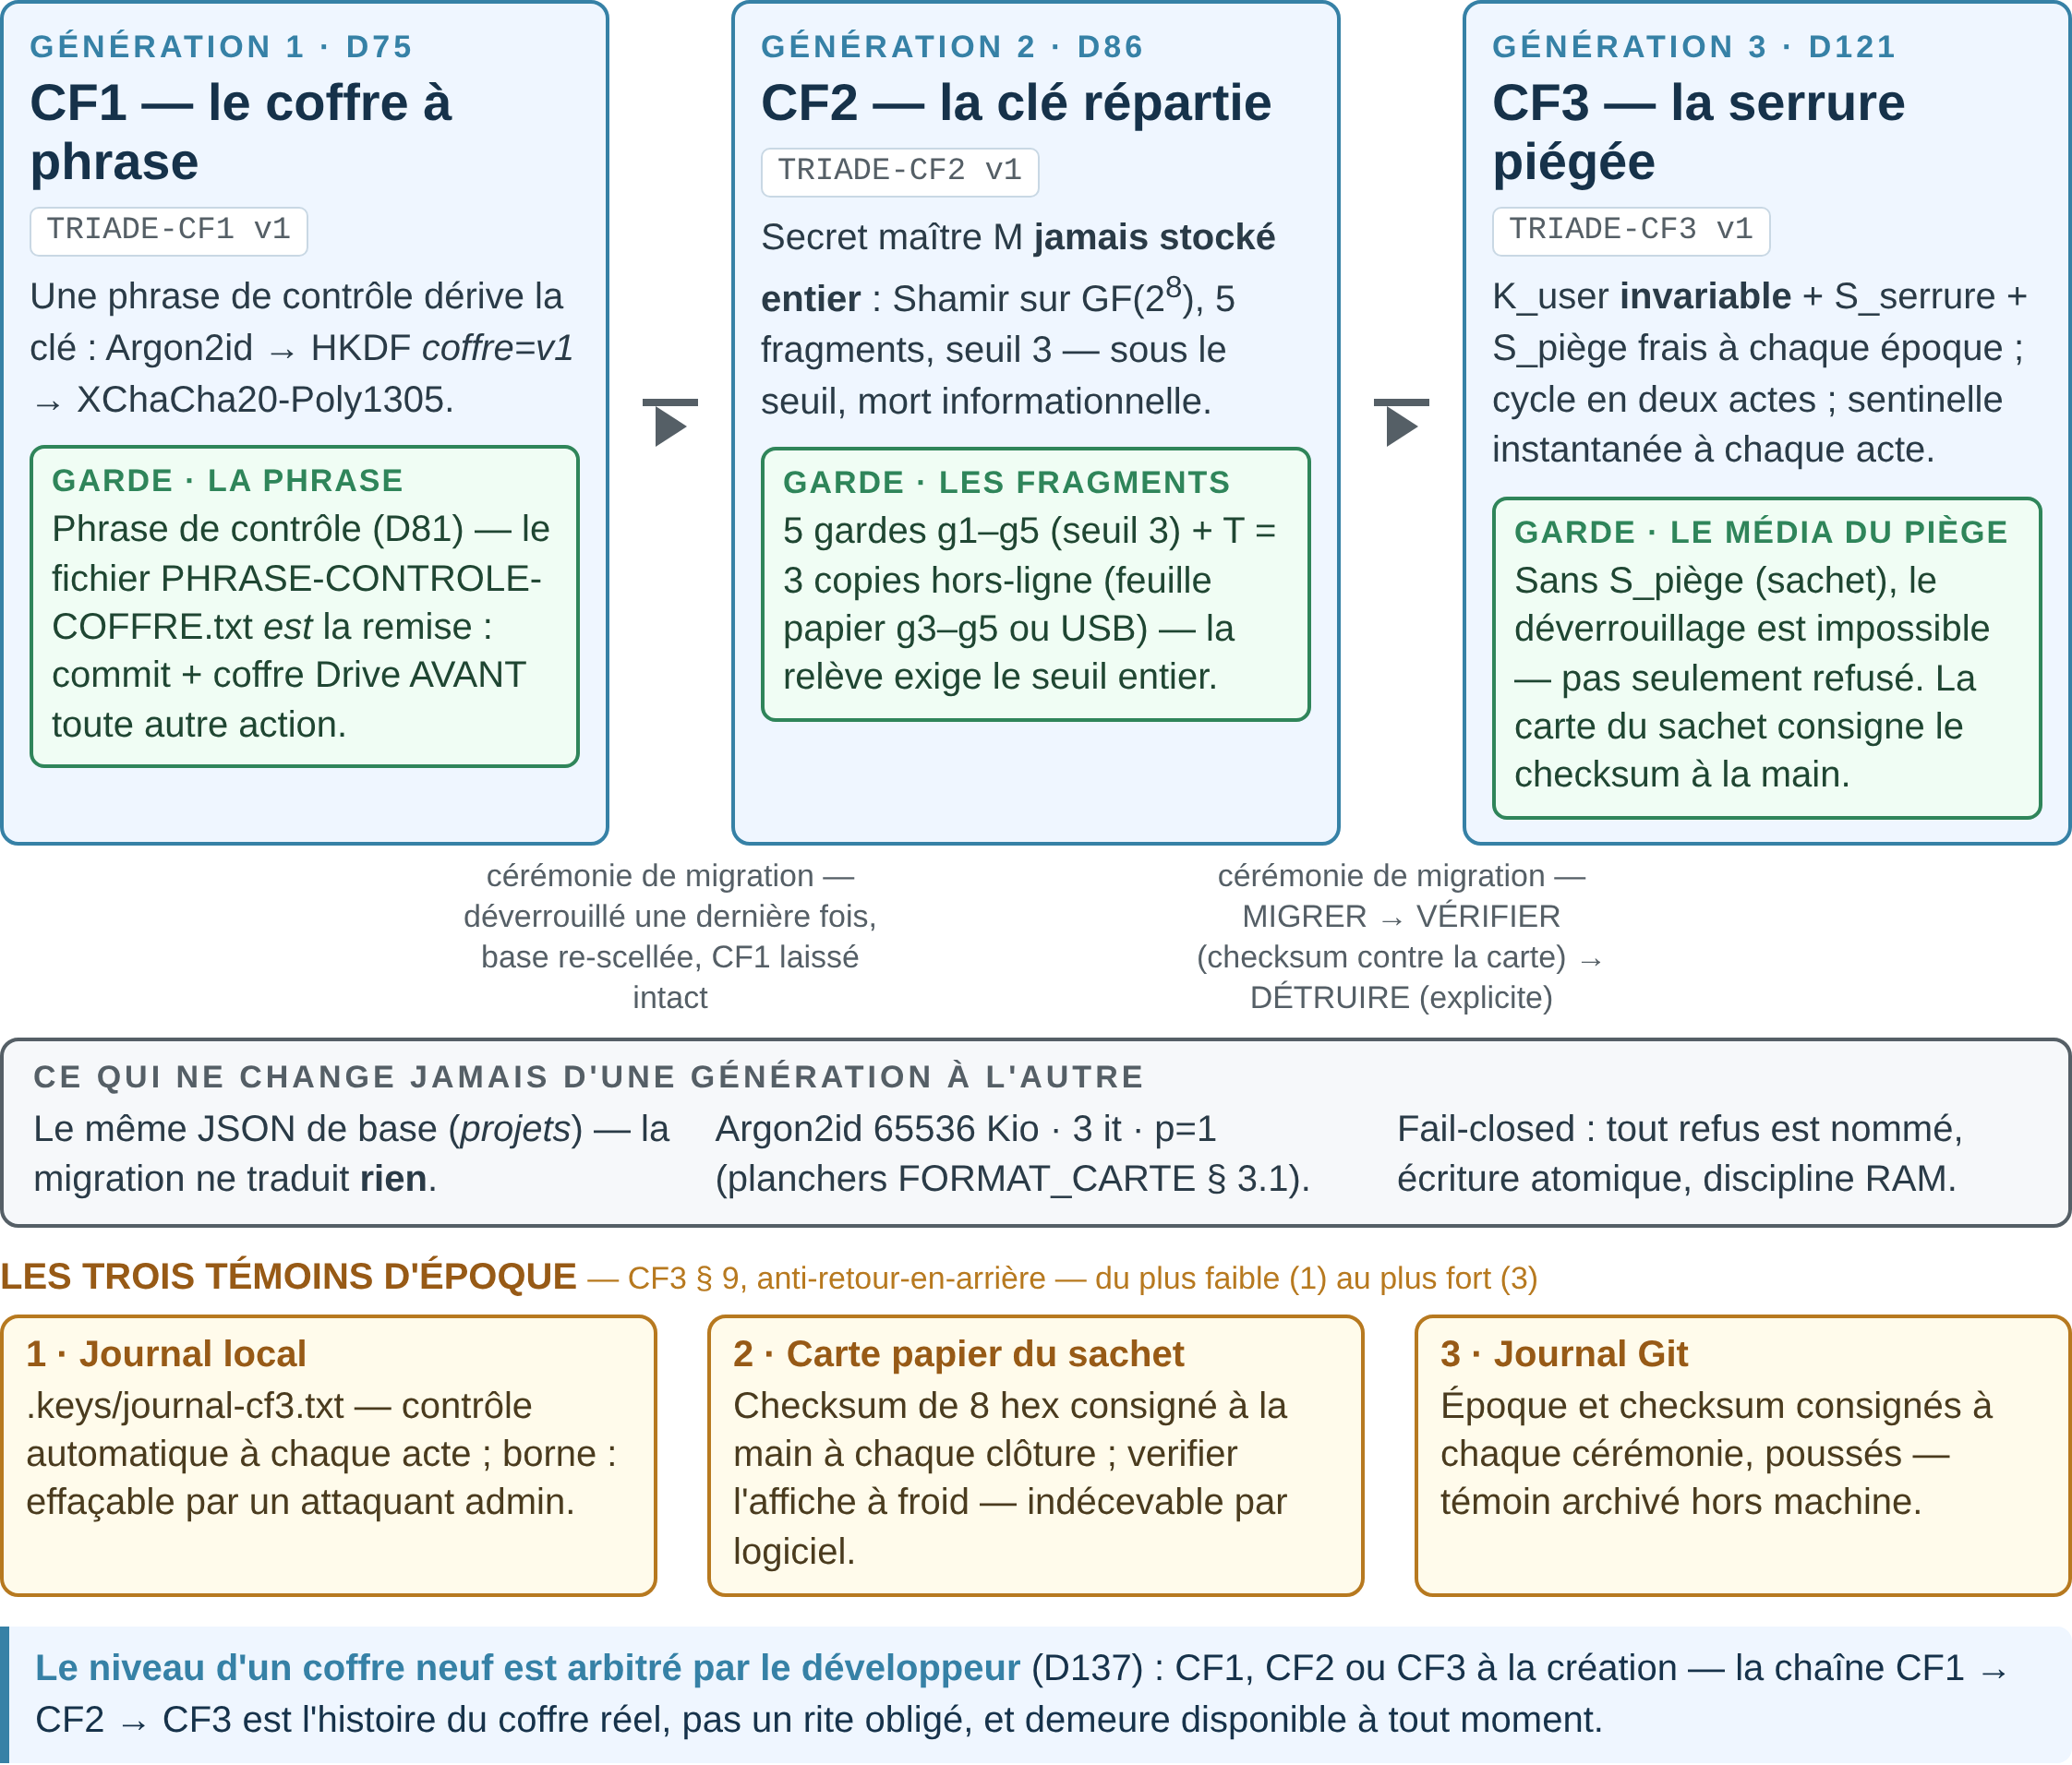
\includegraphics[width=\textwidth, max height=0.62\textheight]{chaine_cf}
\caption{La chaîne du coffre-fort : trois générations, leurs gardes, les trois témoins
d'époque. Le niveau d'un coffre neuf est arbitré par le développeur (D137) ; la chaîne
de migration est l'histoire du coffre réel — et demeure disponible à tout moment.}
\label{fig:chaine}
\end{figure}

\begin{table}[htbp]
\centering\small
\caption{Les cérémonies de la souveraineté — qui fait quoi, et la preuve attendue.}
\label{tab:ceremonies}
\begin{tabularx}{\textwidth}{@{}l Y Y@{}}
\toprule
\textbf{Cérémonie} & \textbf{Gestes} & \textbf{Preuve} \\
\midrule
Sceau de l'Intention (D87/D126) & \code{preparer} (le dépôt écrit \code{a-signer.txt}) ;
cérémonie hors-ligne \code{signer} (clé physique) ; \code{deposer} (chaque signature
vérifiée AVANT écriture) ; \code{verifier} & quatorze arbres VERTS, code 0 ; commit poussé \\
CF1 $\to$ CF2 (D106) & phrase de contrôle (la reconstitution à froid du
séquestre la fournit — jamais un fichier au dépôt, D223) ; \code{migrer} ;
cinq gardes posées ; T = 3 copies hors-ligne (feuille g3--g5 ou USB) ; contrôle de
relecture ; liste blanche & CF2 \code{verifier} VERT ; CF1 laissé intact \\
CF2 $\to$ CF3 (D121/D127) & onglet MIGRER (conteneur CF2, gardes, \emph{média du piège
requis}, phrase deux fois) ; onglet VÉRIFIER (checksum contre la carte du sachet) ;
onglet DÉTRUIRE (case explicite, après recoupement) & époque 1, checksum 8 hex noté sur
la carte ; verdict à froid VERT (recommandé : re-exécution machine froide) \\
Clôture CF3 (usage courant) & acte I : ouverture, média débranché ; session sur le
brouillon ; acte II : phrase retapée, moitiés fraîches, époque N+1, re-lecture à froid
du staging & checksum affiché, ligne sur la carte du sachet ; journal Git consigné \\
Destruction locale (\code{bruler}) & commande explicite
\code{--oui-je-comprends} ; trois passes + PV & PV nommé dans \code{.keys/pv-cf3/} ;
fragments et médias \emph{jamais} touchés \\
\bottomrule
\end{tabularx}
\end{table}

\subsection{Le maître de cérémonie graphique et le trio D122}\label{sec:gui}

Les cérémonies sont conduites par le \textbf{maître de cérémonie graphique}
(\code{v06/ceremonie\_gui.py} pour le sceau et CF2 ; \code{v06/migration\_cf3\_gui.py}
pour CF2 $\to$ CF3) : zéro ligne de commande, un fichier, deux profils (repo git ou
dossier local). Le GUI est un \emph{relais} : il ne réimplémente rien — il lance
\code{coffre\_cf2.py} / \code{coffre\_cf3.py} / \code{sceau\_I.py} et croise le code de
sortie \emph{et} la marque de verdict dans le flux (un enfant menteux est rouge, un
enfant muet est sans verdict). La phrase passe par STDIN, jamais en ligne de commande,
jamais affichée, jamais dans un rapport. Chaque module à tester porte le \textbf{trio
D122} : une GUI, une boîte noire locale horodatée (gitignorée, muette si le disque
refuse — témoin, pas dépendance), un bouton « Envoyer le rapport ». L'habit a appris du
terrain : cahier numéroté comme le fil (D128), pilier droit permanent — le fil d'étapes
et le journal visibles quel que soit l'onglet (D129), un bouton d'attachement par page
(D131), disposition en grille — chaque bouton « Parcourir » sur la ligne de son champ
(D132).

\subsection{Le kit Drive — identité par construction (D130)}\label{sec:kit}

Les cérémonies s’arment depuis le dépôt \emph{ou} depuis le kit du dossier
\code{/Cérémonie} du Drive. Depuis D130, le \code{v06/} du kit est déployé depuis
\code{git ls-files v06/} — la même source que le miroir, lue dans le même arbre de
travail : \textbf{identité octet pour octet par construction}, \code{I/} et
\code{sceau-I/} inclus (preuves publiques du sceau, aucun secret). Le hook post-commit
porte le miroir \emph{puis} le kit dans le même geste — un échec kit ne bloque jamais le
miroir ni le commit, chaque retour est journalisé. Le \code{MANIFESTE.txt} du kit porte
le commit de référence et les empreintes : un kit périmé se \emph{lit}, ne se devine
pas. La racine du kit porte les lanceurs (\code{lancer\_ceremonie},
\code{lancer\_autotest\_cf3}, \code{lancer\_migration\_cf3} — \code{.bat} Windows,
\code{.sh} POSIX) aux conventions D118 : \code{v06/} d'abord, copie plate en repli,
refus nommé sans cible.

\subsection{La preuve terrain de la chaîne réelle (30--31 octobre 2026)}\label{sec:preuveterrain}

Le coffre réel du développeur a parcouru la chaîne entière, rapport de boîte noire à
l'appui : CF1 \code{statut} VERT (conteneur trouvé, en-tête TRIADE-CF1 v1, Argon2id) ;
CF1 \code{verifier} INTÈGRE ; phrase de contrôle changée pour la sienne (D110 —
re-chiffrement, nouveau sel, l'ancienne inopérante) ; un premier \code{migrer} CF2
refusé nommément (« phrase de contrôle divergente » — la remise D81 n'était pas encore
remplacée, la garde d'époque amendée D223 : le fail-closed a travaillé, la cérémonie a été rejouée) ; CF2 né — cinq
fragments sous \code{.keys/gardes-cf2} (seuil 3), CF1 intact, porte D120 posée en ère
sans moteur ; export de la feuille (trois fragments, gardes g3--g5, tags vérifiés avant
impression) ; puis la migration CF3 : \code{migrer} VERT (base re-scellée, schéma
identique — rien à traduire ; piège posé sur le média ; re-lecture à froide verte ;
époque 1, checksum \code{0cc89a96}, conteneur CF2 laissé intact) et \code{verifier} VERT
deux fois, checksum identique — le recoupement machine est fait. La destruction du
conteneur CF2 (acte 4) est un geste \emph{explicite} du maître, après recoupement sur
machine froide : jamais l'ancien avant le vert du neuf. Observation honnête consignée à
la passation : l'empreinte du \code{coffre\_fort.py} mesurée au clone terrain
(\code{299fd124…}) diverge de celle du dépôt (\code{8c79263b…}) — à recouper au
prochain \code{git pull} (\code{git status}) ; le fichier ne sert qu'à la migration
CF1 $\to$ CF2, déjà accomplie.

\subsection{Les cérémonies d'ère du sceau de l'Intention (5 novembre 2026)}\label{sec:ceremoniesere}

Le sceau a traversé deux cérémonies d'ère en un jour, chacune née d'un garde qui
refusait. \textbf{Ère M8} : l'ouverture du domaine \code{sys} avait étendu le
registre figé m0 et créé l'arbre m8 — le garde a nommé la dette AVANT tout build
(D162 : un diff d'intention non signé ; la clé hors-ligne du développeur requise,
le laboratoire ne signe jamais à sa place) ; le kit de cérémonie servi au dossier
\code{/Cérémonie} du Drive (la remise, le LISEZMOI pas à pas, la règle d'or
« JAMAIS generer »), la cérémonie passée sur pièces : douze arbres, les dix
inchangés rendant les MÊMES signatures que celles du 04/11 (la preuve D163 de la
réutilisation de la clé, sans jamais voir la clé privée), le garde repassé VERT
12/12 — puis le build \code{0.9.0-dev.1} né, déterministe d'un poste à l'autre.
\textbf{Ère M9} : la dette fut nommée À LA NAISSANCE (D166, règle 8) ; le geste
des 24 spécifications ayant bougé l'arbre, la charge fut RÉGÉNÉRÉE au geste de la
cérémonie (D168 : la charge de l'ouverture était périmée — une remise signée
dessus aurait laissé l'arbre divergé APRÈS installation) ; le développeur signa
hors ligne la remise de TREIZE arbres et déposa \code{signatures-I.txt} et
\code{cle-publique-I.txt} au coffre \code{/test} ; le laboratoire rapatrie,
recoupe — la clé déposée égale l'ancre \code{173fae9c…}, les ONZE arbres
inchangés rendent les signatures de l'ère M8, m0 re-signé, tls13 arbre neuf, les
empreintes vivantes égales la remise, chaque signature vérifiée Ed25519 — puis
installe canoniquement (tout vérifié AVANT toute écriture) et le garde est
repassé VERT 13/13, l'état « reelle » tenant. La règle qui en découle : la
cérémonie d'ère n'est pas une formalité de documentation — c'est le geste qui
rend le build de l'ère possible, et il suit le calendrier du garde, jamais
l'inverse. \textbf{L'ère du TGN (le domaine \code{loupe}, D171/D175)} a suivi la même
discipline : la dette fut nommée à la naissance de la couche I (D171, règle 8), la
notation des 18 blocs s'accomplit sous elle — quatre chantiers, la table de routage
de loupe-09 étendue en révision nommée sans cascade — AUCUN build avant la
cérémonie (le miroir des ères M8/M9) : LA CÉRÉMONIE EST PASSÉE SUR PIÈCES (D177 :
le garde à QUATORZE arbres), le build est NÉ, ONZE RUNS l'ont vécu — la balise
\code{loupe 0.1.0} est SCELLÉE (D178) : l'ère du TGN est ACCOMPLIE. Le kit de cérémonie vit au dossier
\code{/Cérémonie} du Drive (la remise FRAÎCHE des quatorze arbres — la charge se
prépare AU GESTE de la cérémonie, D168 : les empreintes bougent avec chaque
révision de spécification — le LISEZMOI pas à pas, la règle d'or « JAMAIS generer »)
: le développeur signe hors ligne à la clé du 04/11 (l'ancre de toutes les ères),
ramène \code{signatures-I.txt} et \code{cle-publique-I.txt} au coffre \code{/test}
; le laboratoire rapatrie, recoupe (l'ancre de clé, les arbres inchangés rendant
les MÊMES signatures par le déterminisme Ed25519, m0 re-signé au registre étendu,
l'arbre \code{loupe} neuf), installe canoniquement — et le garde passe à QUATORZE
arbres VERTS : le build de Loupe peut naître.

\subsection{La frontière des secrets — git, \code{.keys}, sachet}\label{sec:frontiere}

La souveraineté vit de frontières \emph{lisibles} : chaque support porte ce qu'il doit
porter, jamais plus.

\begin{table}[htbp]
\centering\small
\caption{La frontière des supports — ce qui vit où, et pourquoi.}
\label{tab:frontiere}
\begin{tabularx}{\textwidth}{@{}l Y Y@{}}
\toprule
\textbf{Support} & \textbf{Ce qu'il porte} & \textbf{Ce qu'il ne porte JAMAIS} \\
\midrule
Dépôt git (poussé) & le code, la SPEC signée (\code{v06/I/}), les preuves publiques du
sceau, le journal de travail — la phrase de contrôle n'y vit plus (amendée D223 : le
séquestre 5/3 la porte, la reconstitution à froid de TROIS parts ; l'historique
D81 du passé git demeure à vie, inopérant par la rotation) & aucun conteneur de coffre
(\code{/.keys/} gitignoré), aucun fragment, aucune graine \\
\code{.keys/} du clone & conteneurs CF1/CF2/CF3, gardes CF2 (5 fragments), config,
journaux et PV locaux, miroir d'époque & jamais dans git — le dossier entier est
gitignoré (ligne 28 du \code{.gitignore}) \\
Le sachet (média séparé) & pièges d'époque (\code{piege-CF3-epoque-N.txt}), T copies
hors-ligne des fragments, la carte papier & jamais branché pendant une session de
travail — le geste de débranchement est consigné au journal de cérémonie \\
Le Drive (miroir + kit) & le dépôt complet en miroir, le kit de cérémonie
(\code{v06/} identique au miroir par construction, D130), le conteneur CF1 de secours &
aucune graine de clé I (le dépôt ne voit que la clé publique) \\
\bottomrule
\end{tabularx}
\end{table}

L'extrait du journal de la migration réelle (boîte noire du GUI, 30/10/2026) —
l'évidence, pas la paraphrase :

\begin{lstlisting}
[CF3-migration] CF2 deverrouille une derniere fois (porte D120 honoree) :
    C:\...\triade\.keys\coffre_cf2.bin
[CF3-migration] base re-scellee sous CF3 (schema identique - rien a traduire) :
    C:\...\triade\.keys\coffre_cf3.bin (epoque 1)
[CF3-migration] piege pose sur le media : D:/piege-CF3-epoque-1.txt
[CF3-migration] re-lecture a froid du scellage : VERTE
[CF3-migration] VERDICT : VERT - epoque 1, checksum 0cc89a96 (1 projet(s))
    - notez-le sur la carte du sachet (spec  9)
[CF3-migration] conteneur CF2 laisse INTACT : C:\...\triade\.keys\coffre_cf2.bin
--- VERDICT migration (actes 1-3) : VERT (code de sortie 0,
    marque « VERDICT : VERT » vue dans le flux)
\end{lstlisting}

\subsection{Référence des commandes}\label{sec:commandes}

Les vérités vivantes que les GUI relaient — la CLI reste la référence (le GUI ne
réimplémente rien) :

\begin{table}[htbp]
\centering\small
\caption{Les commandes du coffre et du sceau (CLI de référence).}
\label{tab:commandes}
\begin{tabularx}{\textwidth}{@{}l >{\raggedright\arraybackslash}p{4.3cm} Y@{}}
\toprule
\textbf{Outil} & \textbf{Commande} & \textbf{Rôle} \\
\midrule
\code{coffre\_cf3.py} & \code{init} & coffre neuf : époque 1, sel et moitiés posés,
piège Nº 1 sur le média \\
 & \code{ouvrir} & acte I : sentinelle + verdict, brouillon sous K\_session \\
 & \code{verifier} & verdict à froid (sentinelle complète, aucune écriture) —
l'outil du recoupement humain \\
 & \code{statut} & étiquette seule — aucune clé dérivée, aucune phrase exigée \\
 & \code{fermer} & acte II : moitiés fraîches, époque N+1, re-lecture à froid du
staging, remplacement atomique \\
 & \code{bruler} & destruction locale MANUELLE (\code{--oui-je-comprends}) — trois
passes + PV \\
 & \code{migrer} & cérémonie CF2 $\to$ CF3 : actes 1--3, CF2 laissé intact \\
 & \code{detruire-cf2} & acte 4 : destruction EXPLICITE du conteneur CF2 (garde
fail-closed si CF3 absent) \\
 & \code{autotest} & autocontrôles sur répertoires temporaires — aucun coffre réel
touché \\
\code{coffre\_cf2.py} & \code{init · migrer · verifier · statut · lister} ; \code{obtenir · ajouter ·
retirer · restaurer · bruler} ; \code{etat-fragments · autotest} & le miroir CF1 de
ces gestes, sur la clé répartie — le détail vit dans la spec scellée CF2 § 8 \\
\code{sceau\_I.py} & \code{preparer · deposer · signer-test · verifier · etat} &
l'intention : prépare la charge à signer, dépose une remise vérifiée, garde le dépôt
(codes 0/10/11/12) \\
\code{ceremonie\_hors\_ligne.py} & \code{generer · signer · verifier} & la cérémonie
air-gap (stdlib seule) : graine, signatures, audit autonome \\
\bottomrule
\end{tabularx}
\end{table}

\paragraph{Cycle de vie d'un coffre neuf.} \code{init} (époque 1, média du piège
désigné dès le premier jour) ; usage courant en cycles \code{ouvrir} /
\code{fermer} — chaque clôture ajoute une ligne à la carte du sachet et incrémente
l'époque ; \code{verifier} à froid après toute doute (recommandé : machine froide le
lendemain d'une cérémonie) ; \code{bruler} le jour où le coffre doit mourir — jamais
avant d'avoir constitué la relève (sachet complet). Les cérémonies de migration
(\code{migrer} CF1 $\to$ CF2 puis CF2 $\to$ CF3, \code{detruire-cf2} en acte explicite)
sont l'histoire d'un coffre né avant sa génération de serrure — un coffre né CF3 ne les
connaît jamais.
